\documentclass[11pt, oneside]{article}   	% use "amsart" instead of "article" for AMSLaTeX format
\usepackage{geometry}                		% See geometry.pdf to learn the layout options. There are lots.
\geometry{letterpaper}                   		% ... or a4paper or a5paper or ... 
%\geometry{landscape}                		% Activate for for rotated page geometry
%\usepackage[parfill]{parskip}    		% Activate to begin paragraphs with an empty line rather than an indent
\usepackage{graphicx}				% Use pdf, png, jpg, or eps� with pdflatex; use eps in DVI mode
								% TeX will automatically convert eps --> pdf in pdflatex		
\usepackage{amssymb}
\usepackage{amsmath}
\usepackage{parskip}
\usepackage{color}
\usepackage{hyperref}

\title{scratch pad}
%\author{The Author}
%\section{}
%\subsection*{}
\date{}							% Activate to display a given date or no date

\graphicspath{{/Users/telliott_admin/Dropbox/Tex/png/}}
% \begin{center} 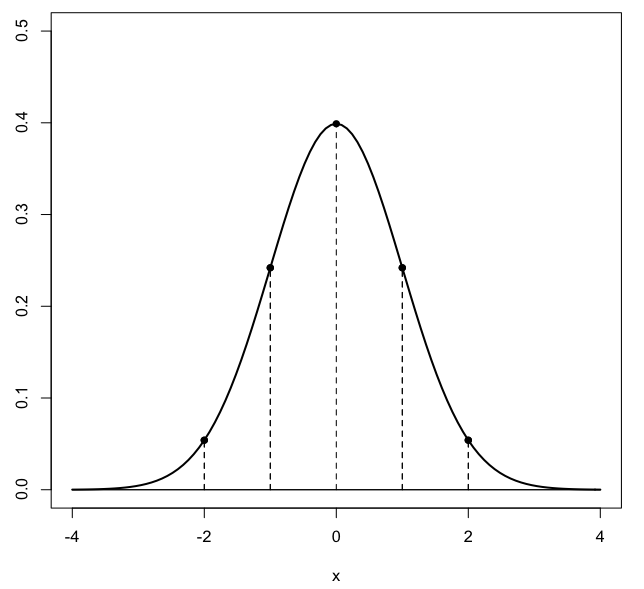
\includegraphics [scale=0.4] {gauss3.png} \end{center}
\begin{document}
\maketitle
\Large
In Chapter 2 of Hamming we find this:  suppose we have the series
\[ \frac{1}{2} + \cos x + \cos 2x + \cos 3x \dots \]
Let $s_n$ be the partial sum of the first $n$ terms
\[ s_n = \frac{1}{2} + \cos x + \cos 2x \dots + \cos nx \]
Recall the addition formulas:
\[ \sin (a + b) = \sin a \cos b + \sin b \cos a \]
\[ \sin (a - b) = \sin a \cos b - \sin b \cos a \]
Subtract
\[ \sin (a + b) - \sin (a - b) = 2 \sin b \cos a \]
\[ \sin b \cos a = \frac{1}{2} \ [ \ \sin (a + b) - \sin (a - b) \ ]  \]
Multiply $s_n$ by $\sin \frac{x}{2}$:
\[ \sin \frac{x}{2} \cdot s_n = \frac{1}{2} \  [ \ \sin \frac{x}{2} + \sin \frac{x}{2} \cdot \cos x + \sin \frac{x}{2} \cdot \cos 2x + \sin \frac{x}{2} \cdot \cos nx \]
Rewrite some typical terms using the result from above:
\[ \sin \frac{x}{2} \cdot \cos x = \frac{1}{2} \ [ \ \sin \frac{3}{2}x - \sin \frac{1}{2}x \ ] \]
\[ \sin \frac{x}{2} \cdot \cos 2x = \frac{1}{2} \ [ \ \sin \frac{5}{2}x - \sin \frac{3}{2}x\ ] \]
Notice that adding the cancellation of $\sin \frac{3}{2}x$.
We have produced a  \emph{telescoping} series:
\[ \sin \frac{x}{2} \cdot s_n =\frac{1}{2} \  [ \ \sin (n + \frac{1}{2}) x \ ] \]
\[ s_n = \frac{\sin (n + \frac{1}{2}) x}{2  \sin \frac{x}{2}} \]
So
\[ \frac{1}{2} + \cos x + \cos 2x \dots  + \cos nx = \frac{\sin (n + \frac{1}{2}) x}{2  \sin \frac{x}{2}} \]
\end{document}  